\documentclass[a4paper]{article}

\usepackage[english]{babel}
\usepackage{amsfonts, amssymb, mathtools, amsthm, amsmath}
\usepackage{graphicx, pgfplots}
\usepackage{bm} 
\usepackage{url}
\usepackage[dvipsnames]{xcolor}
\usepackage{lastpage}
\usepackage{chngcntr}
  \counterwithin{figure}{section}
  \renewcommand{\thefigure}{\thesection.\arabic{figure}}

%loaded last
\usepackage[hidelinks]{hyperref}
\usepackage[nameinlink]{cleveref} 

\usepackage{siunitx}
  \sisetup{exponent-product = \cdot,
    output-decimal-marker = {,}}

%Giles Castelles incfig
\usepackage{import}
\usepackage{xifthen}
\usepackage{pdfpages}
\usepackage{transparent}

\newcommand{\incfig}[2][1]{%
  \def\svgwidth{#1\columnwidth}
  \import{./figures/}{#2.pdf_tex}
}

\setlength{\parindent}{0in}
\setlength{\parskip}{12pt}
\setlength{\oddsidemargin}{0in}
\setlength{\textwidth}{6.5in}
\setlength{\textheight}{8.8in}
\setlength{\topmargin}{0in}
\setlength{\headheight}{18pt}

\usepackage{fancyhdr}
\pagestyle{fancy}

\fancyhead{}
\fancyfoot{}
\fancyfoot[R]{\thepage}
\fancyhead[C]{\leftmark}

\pgfplotsset{compat=newest}

\pgfplotsset{every axis/.append style={
  axis x line=middle,    % put the x axis in the middle
  axis y line=middle,    % put the y axis in the middle
  axis line style={<->,color=black}, % arrows on the axis
}}

\usepackage{thmtools}
\usepackage{tcolorbox}
  \tcbuselibrary{skins, breakable}
  \tcbset{
    space to upper=1em,
    space to lower=1em,
  }

\theoremstyle{definition}

\newtcolorbox[auto counter]{definition}[1][]{%
  breakable,
  colframe=ForestGreen,  %frame color
  colback=ForestGreen!5, %background color
  colbacktitle=ForestGreen!25, %background color for title
  coltitle=ForestGreen!70!black,  %title color
  fonttitle=\bfseries\sffamily, %title font
  left=1em,              %space on left side in box,
  enhanced,              %more options
  frame hidden,          %hide frame
  borderline west={2pt}{0pt}{ForestGreen},  %display left line
  title=Definition \thetcbcounter: #1,
}

\newtcolorbox{greenline}{%
  breakable,
  colframe=ForestGreen,  %frame color
  colback=white,          %remove background color
  left=1em,              %space on left side in box
  enhanced,              %more options
  frame hidden,          %hide frame
  borderline west={2pt}{0pt}{ForestGreen},  %display left line
}

\newtcolorbox[auto counter, number within=section]{dis}[1][]{%
  breakable,
  colframe=NavyBlue,  %frame color
  colback=NavyBlue!5, %background color
  colbacktitle=NavyBlue!25,    %background color for title
  coltitle=NavyBlue!70!black,  %title color
  fonttitle=\bfseries\sffamily, %title font
  left=1em,            %space on left side in box,
  enhanced,            %more options
  frame hidden,        %hide frame
  borderline west={2pt}{0pt}{NavyBlue},  %display left line
  title=Discussion \thetcbcounter: #1
}

\newtcolorbox{blueline}{%
  breakable,
  colframe=NavyBlue,     %frame color
  colback=white,         %remove background
  left=1em,              %space on left side in box,
  enhanced,              %more options
  frame hidden,          %hide frame
  borderline west={2pt}{0pt}{NavyBlue},  %display left line
}

\newtcolorbox{exa}[1][]{%
  breakable,
  colframe=RawSienna,  %frame color
  colback=RawSienna!5, %background color
  colbacktitle=RawSienna!25,    %background color for title
  coltitle=RawSienna!70!black,  %title color
  fonttitle=\bfseries\sffamily, %title font
  left=1em,              %space on left side in box,
  enhanced,              %more options
  frame hidden,          %hide frame
  borderline west={2pt}{0pt}{RawSienna},  %display left line
  title=Example: #1,
}

\newtcolorbox[auto counter, number within=section]{sæt}[1][]{%
  breakable,
  colframe=RawSienna,  %frame color
  colback=RawSienna!5, %background color
  colbacktitle=RawSienna!25,    %background color for title
  coltitle=RawSienna!70!black,  %title color
  fonttitle=\bfseries\sffamily, %title font
  left=1em,              %space on left side in box,
  enhanced,              %more options
  frame hidden,          %hide frame
  borderline west={2pt}{0pt}{RawSienna},  %display left line
  title=Sætning \thetcbcounter: #1,
  before lower={\textbf{Bevis:}\par\vspace{0.5em}},
  colbacklower=RawSienna!25,
}

\newtcolorbox{redline}{%
  breakable,
  colframe=RawSienna,  %frame color
  colback=white,       %Remove background color
  left=1em,            %space on left side in box,
  enhanced,            %more options
  frame hidden,        %hide frame
  borderline west={2pt}{0pt}{RawSienna},  %display left line
}

\newtcolorbox{des}[1][]{%
  breakable,
  colframe=NavyBlue,  %frame color
  colback=NavyBlue!5, %background color
  colbacktitle=NavyBlue!25,    %background color for title
  coltitle=NavyBlue!70!black,  %title color
  fonttitle=\bfseries\sffamily, %title font
  left=1em,              %space on left side in box,
  enhanced,              %more options
  frame hidden,          %hide frame
  borderline west={2pt}{0pt}{NavyBlue},  %display left line
  title=Description of #1,
}

\makeatother
\def\@lecture{}%
\newcommand{\lecture}[3]{
  \ifthenelse{\isempty{#3}}{%
    \def\@lecture{Lecture #1}%
  }{%
    \def\@lecture{Lecture #1: #3}%
  }%
  \subsection*{\makebox[\textwidth][l]{\@lecture \hfill \normalfont\small\textsf{#2}}}
}

\makeatletter

\newcommand{\exercise}[1]{%
 \def\@exercise{#1}%
 \subsection*{Exercise #1}
}

\makeatother

%Format lim the same way in intext and in display
\let\svlim\lim\def\lim{\svlim\limits}

% horizontal rule
\newcommand\hr{
\noindent\rule[0.5ex]{\linewidth}{0.5pt}
}

\author{Noah Rahbek Bigum Hansen}



\title{Prøveeksamen – Termodynamik}
\date{2. Juni 2025}

\begin{document}

\maketitle

\section{Gasturbine kraftvarmeværk} 

\opgave{1} Hvad bliver temperaturen efter kompressoren i punkt [2]?
\bigbreak
Opgaven her er regnet I EES for at kunne benytte stofdatakald. Følgende kode er brugt:

\begin{verbatim}
  T[1] = 15 [C]
  P[1] = 101 [kPa]
  r_p = 10
  eta_kompis = 0,8
  h[1]=enthalpy(Air_ha;T=T[1];P=P[1])
  s[1]=entropy(Air_ha;T=T[1];P=P[1])
   
  P[2]=P[1]*r_p
  h_s[2] = enthalpy(Air_ha;P=P[2]; s=s[1])
   
  h[2] = h[1] + (h_s[2] - h[1])/eta_kompis
  T[2] = temperature(Air_ha; P=P[2]; h=h[2])
\end{verbatim}
Her ses at det antages at luften der løber igennem systemet er metan, at det starter med en temperatur på \qty{15}{\celsius} ved standardtryk. Derudover er opgaven regnet som man ville forvente en opgave af denne type. Resultatet bliver her ifølge EES $T[2] = \qty{344}{\celsius}$.

\opgave{2} Find massestrømmen i brændkammeret?
\bigbreak
Vi antager først og fremmest at brændkammeret er i steady-state, at det er adiabatisk og at kinetiske og potentielle energibidrag er negligerbare. Altså antages at al den tilførte effekt $\dot{Q}_b$ bliver konverteret til en stigning i entalpien for gassen i kredsløbet. Altså:
\[ 
  \dot{Q}_b = \dot{m}_{\mathrm{air}} \left( h[3] - h[2] \right)
.\]
Idet vi antager at der ikke er et trykfald over brændkammeret har vi at $p[3] = p[2]$ derudover er $T[3]$ oplyst i opgaven og derfor kan $h[3]$ findes vha. et stofdatakald i EES. Dermed bliver den samlede EES-kode:

\begin{verbatim}
  P_in = 20000 [MW]
   
  T[1] = 15 [C]
  P[1] = 101 [kPa]
  r_p = 10
  eta_kompis = 0,8
  h[1]=enthalpy(Air_ha;T=T[1];P=P[1])
  s[1]=entropy(Air_ha;T=T[1];P=P[1])
   
  P[2]=P[1]*r_p
  h_s[2] = enthalpy(Air_ha;P=P[2]; s=s[1])
   
  h[2] = h[1] + (h_s[2] - h[1])/eta_kompis
  T[2] = temperature(Air_ha; P=P[2]; h=h[2])
   
   
  T[3] = 900 [C]
  P[3] = P[2]
  h[3] = enthalpy(Air_ha;T=T[3];P=P[3])
   
  P_in = m_dot_air * (h[3] - h[2])
\end{verbatim}
Her giver EES et resultat på $\qty{32,13}{\frac{kg}{s}}$. 

\opgave{3} Hvor meget effekt skal der tilføres i kompressoren?
\bigbreak
Vi antager at kompressoren er i en adiabatisk steady-state. Effekten $\dot{W}_c$ påkrævet er lig massestrøm multipliceret med entalpistigning over kompressoren, som:
\[ 
  \dot{W}_c = \dot{m}_{\mathrm{air}} \left( h[2] - h[1] \right)
.\]
Dette er regnet i EES til $\dot{W}_c = \qty{10813}{kW}$


\opgave{4} Hvad yder turbine-delen?
\bigbreak
For at løse denne opgave findes først den ideele entalpi $h_s[4]$ efter kompressionen såfremt denne var isentalp. Dette kan gøres vha. stofdatakald i EES da isentalpikravet giver $s[3] = s[4]$ og idet det antages at trykfaldet over turbinen bringer luften tilbage til atmosfæretryk $p[4]=p[1]$. 

Dernæst kan den reele entalpi efter kompressionen findes som:
\[ 
  h[4]=h[3]-\eta_{is, t} \left( h[3] - h_s[4] \right)
\]
idet vi kender turbinens virkningsgrad. Slutteligt kan turbinens effekt-output findes som:
\[ 
  \dot{W}_t = \dot{m}_{\mathrm{air}} \left( h[3] - h[4] \right)
.\]
Dette er regnet med denne EES-kode:
\begin{verbatim}
  P_in = 20000 [MW]
   
  T[1] = 15 [C]
  p[1] = 101 [kPa]
  r_p = 10
  eta_kompis = 0,8
  h[1]=enthalpy(Air_ha;T=T[1];P=p[1])
  s[1]=entropy(Air_ha;T=T[1];P=p[1])
   
  p[2]=p[1]*r_p
  h_s[2] = enthalpy(Air_ha;P=p[2]; s=s[1])
   
  h[2] = h[1] + (h_s[2] - h[1])/eta_kompis
  T[2] = temperature(Air_ha; P=p[2]; h=h[2])
  s[2] = enthalpy(Air_ha;P=p[2]; T=T[2])
   
   
  T[3] = 900 [C]
  p[3] = p[2]
  h[3] = enthalpy(Air_ha;T=T[3];P=p[3])
  s[3] = entropy(Air_ha;P=p[3]; T=T[3])
   
  P_in = m_dot_air * (h[3] - h[2])
 
  W_dot_c = m_dot_air * (h[2] - h[1])
 
  eta_turbis = 0,85
 
  p[4] = p[1]
  h_s[4] = enthalpy(Air_ha;P=p[4]; s=s[3])
  h[4] = h[3] - eta_turbis * (h[3] - h_s[4])
  T[4] = temperature(Air_ha; P=p[4]; h=h[4])
  s[4] = entropy(Air_ha; P=p[4]; h=h[4])
 
  W_dot_t = m_dot_air * (h[3]-h[4])
\end{verbatim}
Her giver EES et resultat på $\dot{W}_c = \qty{16076}{kW}$. 

\opgave{5} Skitser processen i et Ts-diagram?
\bigbreak
Vha. samme EES-kode som ovenfor er følgende property plot produceret i EES:
\begin{figure} [ht]
  \centering
  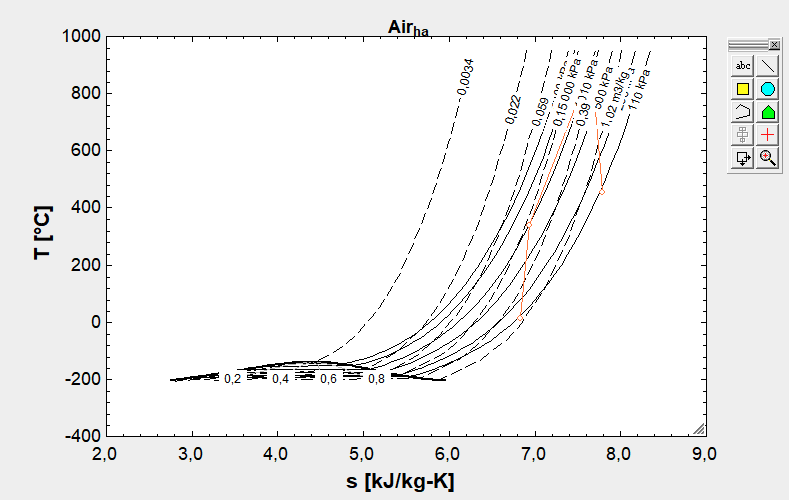
\includegraphics[width=0.5\linewidth]{./figures/p2_1.png}
  \caption{Ts-diagram for processen}
  \label{fig:p2_1}
\end{figure}


\opgave{6} Hvad bliver gasturbinens el-effekt?
\bigbreak
El-effekt outputtet af gasturbinen $W_{el}$ er blot differensen mellem den påkrævede effekt i kompressoren og den genererede effekt i turbinen:
\[ 
W_{\mathrm{el}} = W_t - W_c = \qty{16076}{kW} - \qty{10813}{kW} = \qty{5263}{kW}
.\]
Altså produceres der knap \qty{5263}{kW} i gasturbinen.


\opgave{7} Opstil et skema med de vigtigste tilstandstørrelser for processen.
\bigbreak
Følgende tabel er produceret i EES:
\begin{figure} [ht]
  \centering
  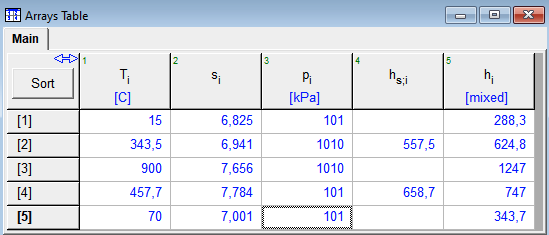
\includegraphics[width=0.5\linewidth]{./figures/p2_2.png}
  \caption{Tabel med relevant data}
  \label{fig:p2_2}
\end{figure}

\opgave{8} Hvad bliver røggastemperaturen efter gasturbinen i punkt [4]?
\bigbreak
I tabellen kan aflæses at røggastemperaturen efter gasturbinen er $T[4] = \qty{458}{\celsius}$. 

\opgave{9} Hvad bliver anlæggets fjernvarmeydelse?
\bigbreak
Fjernvarmeoutputtet kan blot findes som:
\[ 
  Q_{\mathrm{fjv}} = \dot{m}_{\mathrm{air}} \cdot \left( h[4] - h[5] \right)
.\]
Dette er i EES regnet til $Q_{\mathrm{fjv}} = \qty{12957}{kW} $




\end{document}
